\documentclass[../../main.tex]{subfiles}

\begin{document}

\chapter{Figures in \LaTeX}

\section{ Environment For Using Figures}
\lstinputlisting[
    language=TeXish,
    linerange={1-16}
]{\subfix{example_codes/environment_basic_figure.tex}}

\lstinputlisting[
    language=TeX,
    linerange={18-20}
]{\subfix{example_codes/environment_basic_figure.tex}}
\clearpage

\section{ Environment For Box Figures and List figures}
\lstinputlisting[
    language=TeXish,
    linerange={1-15}
]{\subfix{example_codes/environment_figure_box.tex}}

\lstinputlisting[
    language=TeX,
    linerange={17-24}
]{\subfix{example_codes/environment_figure_box.tex}}
\clearpage

\section{ Simple Figures}
% usepackage : graphicx(includegraphics), float(h!), subfiles(subfix), caption 
\begin{figure}[h!]
    \centering  
    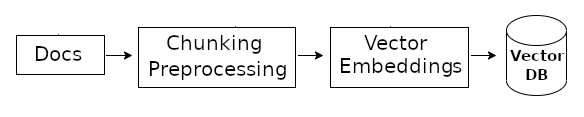
\includegraphics[width=0.6\linewidth]{\subfix{example_codes/img_02.jpg}}
    \caption{A simple example image.}
    \label{fig:simple_image}
\end{figure}}
\lstinputlisting{\subfix{example_codes/basic_figure.tex}}

\section{ Figures in Box, keep in list}

% usepackage : caption
\begin{center}
    % Boxed image
    \fbox{%
      \begin{minipage}{0.6\linewidth}
        \centering  
        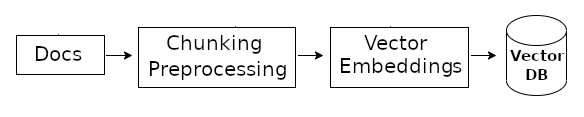
\includegraphics[width=0.9\linewidth]{\subfix{example_codes/img_02.jpg}}
        \captionof{figure}{A simple example image inside a box.}
        \label{fig:simple_boxed_image}
      \end{minipage}
    }
\end{center}}
\lstinputlisting{\subfix{example_codes/figure_box.tex}}
\clearpage

\section{ Importatnt Points to add Figures}
\begin{itemize}
    \item Create environment(template) which take arguments and display image.
    \item Create a seprate tex file that will use the template to display image.
    \item Import the tex file create in above step to your main code.
\end{itemize}
}

\end{document}
